
\noindent\begin{minipage}{\textwidth}
    \begin{table}[H]
        \centering
        \caption{Hiperparâmetros e Resultados do Melhor Modelo - densenet\_v11\_AM\_opt\_aug}
        \vspace{0.2cm}
        \resizebox{\textwidth}{!}{%
            \begin{tabular}{ll | lrrr}
                \hline
                \multicolumn{2}{c|}{\textbf{Hiperparâmetros}} & \multicolumn{4}{c}{\textbf{Métricas por Classe}} \\ \hline
                \textbf{Parâmetro} & \textbf{Valor} & \textbf{Classe} & \textbf{Precisão} & \textbf{Recall} & \textbf{F1-Score} \\ \hline
    Agendador (Patience) & 4 & 31.2 & 0,1867 & 0,7434 & 0,2984 \\ 
Agendador de LR & ReduceLROnPlateau & 31.3 & 0,0000 & 0,0000 & 0,0000 \\ 
Architecture & densenet121 & 31.4 & 0,2941 & 0,0238 & 0,0441 \\ 
Batch Size & 32 & 32.3 & 0,4444 & 0,0816 & 0,1379 \\ 
Data Augmentation & False & 32.4 & 0,0000 & 0,0000 & 0,0000 \\ 
Decaimento de Peso (WD) & 0,0003 & 33.3 & 0,1617 & 0,2539 & 0,1976 \\ 
Dropout & 0,4186 & 41.4 & 0,5000 & 0,0455 & 0,0833 \\ 
Função de Perda & CrossEntropyLoss & 41.5 & 0,0000 & 0,0000 & 0,0000 \\ 
Hidden Units & 256 & 42.4 & 0,0000 & 0,0000 & 0,0000 \\ 
Label Smoothing & 0,1000 & 44.4 & 0,0000 & 0,0000 & 0,0000 \\ 
\cline{3-6} 
Otimizador & AdamW & \textbf{Média (Macro)} & 0,4871 & 0,1885 & 0,1721 \\ 
Taxa de Aprendizado (LR) & 1,51e-04 & \textbf{MCC} & \multicolumn{3}{c}{0,1616} \\ 
Unfreeze Layers & 6 &  & & &  \\ 
            \hline
            \end{tabular}%
        }
    \end{table}

    \begin{figure}[H]
        \centering
        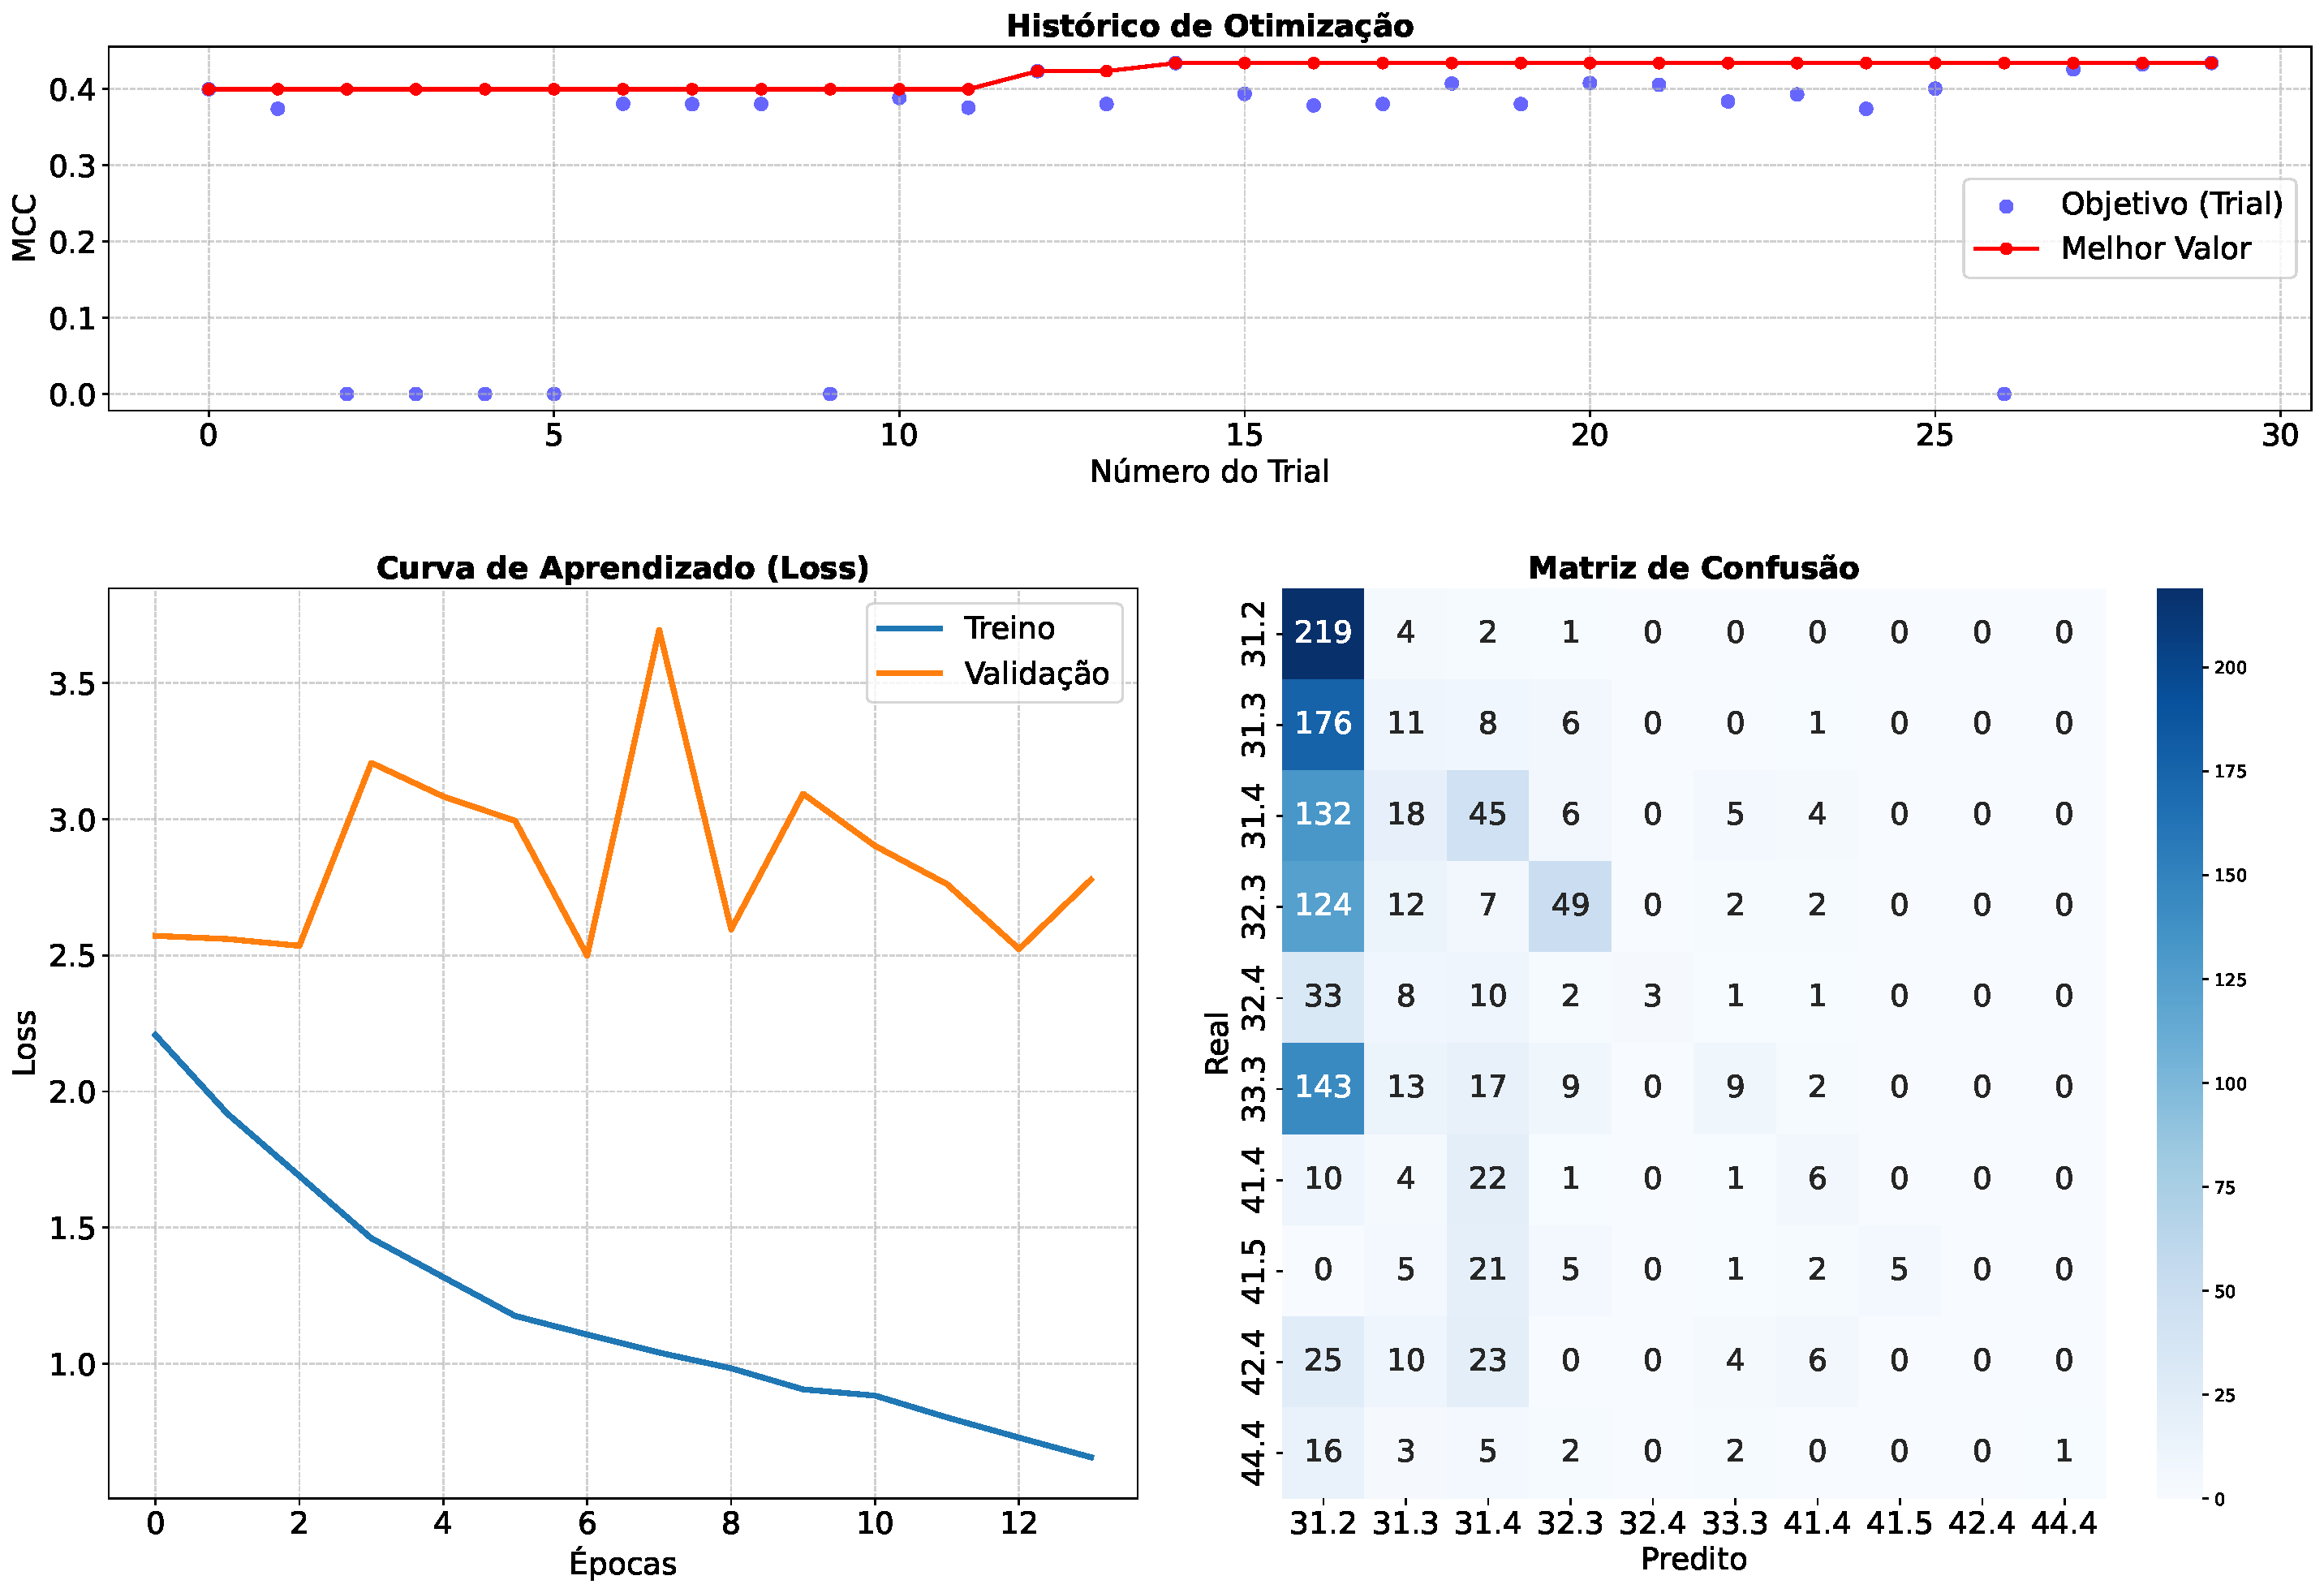
\includegraphics[width=0.85\textwidth]{tex/appendix/experiments/densenet_v11_AM_opt_aug/dashboard_consolidado.pdf}
        \caption{Histórico de Otimização, Curvas de Aprendizado e Matriz de Confusão - densenet\_v11\_AM\_opt\_aug}
    \end{figure}
\end{minipage}
\clearpage
